\documentclass[twoside]{book}

% Packages required by doxygen
\usepackage{fixltx2e}
\usepackage{calc}
\usepackage{doxygen}
\usepackage[export]{adjustbox} % also loads graphicx
\usepackage{graphicx}
\usepackage[utf8]{inputenc}
\usepackage{makeidx}
\usepackage{multicol}
\usepackage{multirow}
\PassOptionsToPackage{warn}{textcomp}
\usepackage{textcomp}
\usepackage[nointegrals]{wasysym}
\usepackage[table]{xcolor}

% Font selection
\usepackage[T1]{fontenc}
\usepackage[scaled=.90]{helvet}
\usepackage{courier}
\usepackage{amssymb}
\usepackage{sectsty}
\renewcommand{\familydefault}{\sfdefault}
\allsectionsfont{%
  \fontseries{bc}\selectfont%
  \color{darkgray}%
}
\renewcommand{\DoxyLabelFont}{%
  \fontseries{bc}\selectfont%
  \color{darkgray}%
}
\newcommand{\+}{\discretionary{\mbox{\scriptsize$\hookleftarrow$}}{}{}}

% Page & text layout
\usepackage{geometry}
\geometry{%
  a4paper,%
  top=2.5cm,%
  bottom=2.5cm,%
  left=2.5cm,%
  right=2.5cm%
}
\tolerance=750
\hfuzz=15pt
\hbadness=750
\setlength{\emergencystretch}{15pt}
\setlength{\parindent}{0cm}
\setlength{\parskip}{3ex plus 2ex minus 2ex}
\makeatletter
\renewcommand{\paragraph}{%
  \@startsection{paragraph}{4}{0ex}{-1.0ex}{1.0ex}{%
    \normalfont\normalsize\bfseries\SS@parafont%
  }%
}
\renewcommand{\subparagraph}{%
  \@startsection{subparagraph}{5}{0ex}{-1.0ex}{1.0ex}{%
    \normalfont\normalsize\bfseries\SS@subparafont%
  }%
}
\makeatother

% Headers & footers
\usepackage{fancyhdr}
\pagestyle{fancyplain}
\fancyhead[LE]{\fancyplain{}{\bfseries\thepage}}
\fancyhead[CE]{\fancyplain{}{}}
\fancyhead[RE]{\fancyplain{}{\bfseries\leftmark}}
\fancyhead[LO]{\fancyplain{}{\bfseries\rightmark}}
\fancyhead[CO]{\fancyplain{}{}}
\fancyhead[RO]{\fancyplain{}{\bfseries\thepage}}
\fancyfoot[LE]{\fancyplain{}{}}
\fancyfoot[CE]{\fancyplain{}{}}
\fancyfoot[RE]{\fancyplain{}{\bfseries\scriptsize Generated by Doxygen }}
\fancyfoot[LO]{\fancyplain{}{\bfseries\scriptsize Generated by Doxygen }}
\fancyfoot[CO]{\fancyplain{}{}}
\fancyfoot[RO]{\fancyplain{}{}}
\renewcommand{\footrulewidth}{0.4pt}
\renewcommand{\chaptermark}[1]{%
  \markboth{#1}{}%
}
\renewcommand{\sectionmark}[1]{%
  \markright{\thesection\ #1}%
}

% Indices & bibliography
\usepackage{natbib}
\usepackage[titles]{tocloft}
\setcounter{tocdepth}{3}
\setcounter{secnumdepth}{5}
\makeindex

% Hyperlinks (required, but should be loaded last)
\usepackage{ifpdf}
\ifpdf
  \usepackage[pdftex,pagebackref=true]{hyperref}
\else
  \usepackage[ps2pdf,pagebackref=true]{hyperref}
\fi
\hypersetup{%
  colorlinks=true,%
  linkcolor=blue,%
  citecolor=blue,%
  unicode%
}

% Custom commands
\newcommand{\clearemptydoublepage}{%
  \newpage{\pagestyle{empty}\cleardoublepage}%
}

\usepackage{caption}
\captionsetup{labelsep=space,justification=centering,font={bf},singlelinecheck=off,skip=4pt,position=top}

%===== C O N T E N T S =====

\begin{document}

% Titlepage & ToC
\hypersetup{pageanchor=false,
             bookmarksnumbered=true,
             pdfencoding=unicode
            }
\pagenumbering{alph}
\begin{titlepage}
\vspace*{7cm}
\begin{center}%
{\Large Pet Behaviour \\[1ex]\large 1.\+0 }\\
\vspace*{1cm}
{\large Generated by Doxygen 1.8.13}\\
\end{center}
\end{titlepage}
\clearemptydoublepage
\pagenumbering{roman}
\tableofcontents
\clearemptydoublepage
\pagenumbering{arabic}
\hypersetup{pageanchor=true}

%--- Begin generated contents ---
\chapter{Namespace Index}
\section{Namespace List}
Here is a list of all documented namespaces with brief descriptions\+:\begin{DoxyCompactList}
\item\contentsline{section}{\hyperlink{namespacebehaviour__controller}{behaviour\+\_\+controller} \\*State machine to control the behaviour of the pet }{\pageref{namespacebehaviour__controller}}{}
\item\contentsline{section}{\hyperlink{namespacemotion__controller}{motion\+\_\+controller} \\*Control the position of the pet in the map respecting the behaviour }{\pageref{namespacemotion__controller}}{}
\item\contentsline{section}{\hyperlink{namespacepointing__gesture__gen}{pointing\+\_\+gesture\+\_\+gen} \\*Pointing gesture generator (a Int\+List) with random delays }{\pageref{namespacepointing__gesture__gen}}{}
\item\contentsline{section}{\hyperlink{namespacesimulator}{simulator} \\*Display pet position and user actions }{\pageref{namespacesimulator}}{}
\item\contentsline{section}{\hyperlink{namespacevoice__command__gen}{voice\+\_\+command\+\_\+gen} \\*Voice command generator (a string) with random delays }{\pageref{namespacevoice__command__gen}}{}
\end{DoxyCompactList}

\chapter{Hierarchical Index}
\section{Class Hierarchy}
This inheritance list is sorted roughly, but not completely, alphabetically\+:\begin{DoxyCompactList}
\item \contentsline{section}{pet\+\_\+map.\+Pet\+Map}{\pageref{classpet__map_1_1PetMap}}{}
\item State\begin{DoxyCompactList}
\item \contentsline{section}{behaviour\+\_\+controller.\+Normal}{\pageref{classbehaviour__controller_1_1Normal}}{}
\item \contentsline{section}{behaviour\+\_\+controller.\+Play}{\pageref{classbehaviour__controller_1_1Play}}{}
\item \contentsline{section}{behaviour\+\_\+controller.\+Sleep}{\pageref{classbehaviour__controller_1_1Sleep}}{}
\end{DoxyCompactList}
\end{DoxyCompactList}

\chapter{Class Index}
\section{Class List}
Here are the classes, structs, unions and interfaces with brief descriptions\+:\begin{DoxyCompactList}
\item\contentsline{section}{\hyperlink{classbehaviour__controller_1_1Normal}{behaviour\+\_\+controller.\+Normal} \\*Class state \hyperlink{classbehaviour__controller_1_1Normal}{Normal} }{\pageref{classbehaviour__controller_1_1Normal}}{}
\item\contentsline{section}{\hyperlink{classpet__map_1_1PetMap}{pet\+\_\+map.\+Pet\+Map} \\*Class Map }{\pageref{classpet__map_1_1PetMap}}{}
\item\contentsline{section}{\hyperlink{classbehaviour__controller_1_1Play}{behaviour\+\_\+controller.\+Play} \\*Class state \hyperlink{classbehaviour__controller_1_1Play}{Play} }{\pageref{classbehaviour__controller_1_1Play}}{}
\item\contentsline{section}{\hyperlink{classbehaviour__controller_1_1Sleep}{behaviour\+\_\+controller.\+Sleep} \\*Class state \hyperlink{classbehaviour__controller_1_1Sleep}{Sleep} }{\pageref{classbehaviour__controller_1_1Sleep}}{}
\end{DoxyCompactList}

\chapter{Namespace Documentation}
\hypertarget{namespacebehaviour__controller}{}\section{behaviour\+\_\+controller Namespace Reference}
\label{namespacebehaviour__controller}\index{behaviour\+\_\+controller@{behaviour\+\_\+controller}}


state machine to control the behaviour of the pet  


\subsection*{Classes}
\begin{DoxyCompactItemize}
\item 
class \hyperlink{classbehaviour__controller_1_1Normal}{Normal}
\begin{DoxyCompactList}\small\item\em class state \hyperlink{classbehaviour__controller_1_1Normal}{Normal} \end{DoxyCompactList}\item 
class \hyperlink{classbehaviour__controller_1_1Play}{Play}
\begin{DoxyCompactList}\small\item\em class state \hyperlink{classbehaviour__controller_1_1Play}{Play} \end{DoxyCompactList}\item 
class \hyperlink{classbehaviour__controller_1_1Sleep}{Sleep}
\begin{DoxyCompactList}\small\item\em class state \hyperlink{classbehaviour__controller_1_1Sleep}{Sleep} \end{DoxyCompactList}\end{DoxyCompactItemize}
\subsection*{Functions}
\begin{DoxyCompactItemize}
\item 
\mbox{\Hypertarget{namespacebehaviour__controller_a35bfb7eb5f65e03cc1eb8e69d13c10fa}\label{namespacebehaviour__controller_a35bfb7eb5f65e03cc1eb8e69d13c10fa}} 
def {\bfseries main} ()
\end{DoxyCompactItemize}
\subsection*{Variables}
\begin{DoxyCompactItemize}
\item 
\mbox{\Hypertarget{namespacebehaviour__controller_a5b870432f520ae88808f78b28df218bf}\label{namespacebehaviour__controller_a5b870432f520ae88808f78b28df218bf}} 
{\bfseries pub\+\_\+state} = rospy.\+Publisher(\char`\"{}/behaviour\char`\"{},String,queue\+\_\+size=5)
\end{DoxyCompactItemize}


\subsection{Detailed Description}
state machine to control the behaviour of the pet 
\hypertarget{namespacemotion__controller}{}\section{motion\+\_\+controller Namespace Reference}
\label{namespacemotion__controller}\index{motion\+\_\+controller@{motion\+\_\+controller}}


control the position of the pet in the map respecting the behaviour  


\subsection*{Functions}
\begin{DoxyCompactItemize}
\item 
def \hyperlink{namespacemotion__controller_a8a8e2917c2712d2afb49419c6aa1379d}{get\+\_\+random\+\_\+position} ()
\begin{DoxyCompactList}\small\item\em function get\+\_\+random\+\_\+position \end{DoxyCompactList}\item 
def \hyperlink{namespacemotion__controller_ad8b145f02fe5a2855d870dcba1fcc55c}{get\+\_\+position} (position)
\begin{DoxyCompactList}\small\item\em function get\+\_\+position \end{DoxyCompactList}\item 
def \hyperlink{namespacemotion__controller_a40fc810329104a6303a97e168e610c49}{get\+\_\+behaviour} (state)
\begin{DoxyCompactList}\small\item\em function get\+\_\+behaviour \end{DoxyCompactList}\item 
def \hyperlink{namespacemotion__controller_ad0d79d45374055e40016deb85d442b68}{move\+\_\+normal} ()
\begin{DoxyCompactList}\small\item\em function move\+\_\+normal \end{DoxyCompactList}\item 
def \hyperlink{namespacemotion__controller_aa7f1f1344aaf5e6d83f0969cd68f4d85}{move\+\_\+sleep} ()
\begin{DoxyCompactList}\small\item\em function move\+\_\+sleep \end{DoxyCompactList}\item 
def \hyperlink{namespacemotion__controller_a539bdfd40405e3ecb739d369e9ab8c5a}{move\+\_\+to\+\_\+person} ()
\begin{DoxyCompactList}\small\item\em function move\+\_\+to\+\_\+person \end{DoxyCompactList}\item 
def \hyperlink{namespacemotion__controller_af23057c8b423f4c23d2d6b61fa38c2f6}{move\+\_\+to\+\_\+goal} ()
\begin{DoxyCompactList}\small\item\em function move\+\_\+to\+\_\+goal \end{DoxyCompactList}\item 
\mbox{\Hypertarget{namespacemotion__controller_a6166ed8edc1044e84dbd14b656004666}\label{namespacemotion__controller_a6166ed8edc1044e84dbd14b656004666}} 
def \hyperlink{namespacemotion__controller_a6166ed8edc1044e84dbd14b656004666}{main} ()
\begin{DoxyCompactList}\small\item\em main function \end{DoxyCompactList}\end{DoxyCompactItemize}
\subsection*{Variables}
\begin{DoxyCompactItemize}
\item 
\mbox{\Hypertarget{namespacemotion__controller_a8ac02bda1a8eb65904002041626fc5c4}\label{namespacemotion__controller_a8ac02bda1a8eb65904002041626fc5c4}} 
\hyperlink{namespacemotion__controller_a8ac02bda1a8eb65904002041626fc5c4}{pet\+\_\+map} = Pet\+Map()
\begin{DoxyCompactList}\small\item\em initialization of the map and variables \end{DoxyCompactList}\item 
\mbox{\Hypertarget{namespacemotion__controller_ad0c236105be213f01f26f9b82746bad3}\label{namespacemotion__controller_ad0c236105be213f01f26f9b82746bad3}} 
{\bfseries goal\+\_\+position} = None
\item 
\mbox{\Hypertarget{namespacemotion__controller_a59855c6c759e43e15becff8da2993298}\label{namespacemotion__controller_a59855c6c759e43e15becff8da2993298}} 
{\bfseries behaviour} = None
\item 
\mbox{\Hypertarget{namespacemotion__controller_ac7a2319b315fc7099ca438419541baff}\label{namespacemotion__controller_ac7a2319b315fc7099ca438419541baff}} 
{\bfseries timescale} = rospy.\+get\+\_\+param(\textquotesingle{}timescale\textquotesingle{})
\item 
\mbox{\Hypertarget{namespacemotion__controller_a88e04e4993ea68310131342873cd53a7}\label{namespacemotion__controller_a88e04e4993ea68310131342873cd53a7}} 
bool {\bfseries home} = False
\item 
\mbox{\Hypertarget{namespacemotion__controller_adc4eb7fa2ec8ead019615208248fe2f3}\label{namespacemotion__controller_adc4eb7fa2ec8ead019615208248fe2f3}} 
{\bfseries pub} = rospy.\+Publisher(\char`\"{}/actual\+\_\+position\char`\"{},Int\+List,queue\+\_\+size=5)
\item 
\mbox{\Hypertarget{namespacemotion__controller_a3bc548adde90d1979cbb1c2823d411dd}\label{namespacemotion__controller_a3bc548adde90d1979cbb1c2823d411dd}} 
{\bfseries sub} = None
\end{DoxyCompactItemize}


\subsection{Detailed Description}
control the position of the pet in the map respecting the behaviour 

\subsection{Function Documentation}
\mbox{\Hypertarget{namespacemotion__controller_a40fc810329104a6303a97e168e610c49}\label{namespacemotion__controller_a40fc810329104a6303a97e168e610c49}} 
\index{motion\+\_\+controller@{motion\+\_\+controller}!get\+\_\+behaviour@{get\+\_\+behaviour}}
\index{get\+\_\+behaviour@{get\+\_\+behaviour}!motion\+\_\+controller@{motion\+\_\+controller}}
\subsubsection{\texorpdfstring{get\+\_\+behaviour()}{get\_behaviour()}}
{\footnotesize\ttfamily def motion\+\_\+controller.\+get\+\_\+behaviour (\begin{DoxyParamCaption}\item[{}]{state }\end{DoxyParamCaption})}



function get\+\_\+behaviour 

subscriber callback to the behaviour topic \mbox{\Hypertarget{namespacemotion__controller_ad8b145f02fe5a2855d870dcba1fcc55c}\label{namespacemotion__controller_ad8b145f02fe5a2855d870dcba1fcc55c}} 
\index{motion\+\_\+controller@{motion\+\_\+controller}!get\+\_\+position@{get\+\_\+position}}
\index{get\+\_\+position@{get\+\_\+position}!motion\+\_\+controller@{motion\+\_\+controller}}
\subsubsection{\texorpdfstring{get\+\_\+position()}{get\_position()}}
{\footnotesize\ttfamily def motion\+\_\+controller.\+get\+\_\+position (\begin{DoxyParamCaption}\item[{}]{position }\end{DoxyParamCaption})}



function get\+\_\+position 

subscriber callback position \mbox{\Hypertarget{namespacemotion__controller_a8a8e2917c2712d2afb49419c6aa1379d}\label{namespacemotion__controller_a8a8e2917c2712d2afb49419c6aa1379d}} 
\index{motion\+\_\+controller@{motion\+\_\+controller}!get\+\_\+random\+\_\+position@{get\+\_\+random\+\_\+position}}
\index{get\+\_\+random\+\_\+position@{get\+\_\+random\+\_\+position}!motion\+\_\+controller@{motion\+\_\+controller}}
\subsubsection{\texorpdfstring{get\+\_\+random\+\_\+position()}{get\_random\_position()}}
{\footnotesize\ttfamily def motion\+\_\+controller.\+get\+\_\+random\+\_\+position (\begin{DoxyParamCaption}{ }\end{DoxyParamCaption})}



function get\+\_\+random\+\_\+position 

get a random position on the map \mbox{\Hypertarget{namespacemotion__controller_ad0d79d45374055e40016deb85d442b68}\label{namespacemotion__controller_ad0d79d45374055e40016deb85d442b68}} 
\index{motion\+\_\+controller@{motion\+\_\+controller}!move\+\_\+normal@{move\+\_\+normal}}
\index{move\+\_\+normal@{move\+\_\+normal}!motion\+\_\+controller@{motion\+\_\+controller}}
\subsubsection{\texorpdfstring{move\+\_\+normal()}{move\_normal()}}
{\footnotesize\ttfamily def motion\+\_\+controller.\+move\+\_\+normal (\begin{DoxyParamCaption}{ }\end{DoxyParamCaption})}



function move\+\_\+normal 

movement in the N\+O\+R\+M\+AL state \mbox{\Hypertarget{namespacemotion__controller_aa7f1f1344aaf5e6d83f0969cd68f4d85}\label{namespacemotion__controller_aa7f1f1344aaf5e6d83f0969cd68f4d85}} 
\index{motion\+\_\+controller@{motion\+\_\+controller}!move\+\_\+sleep@{move\+\_\+sleep}}
\index{move\+\_\+sleep@{move\+\_\+sleep}!motion\+\_\+controller@{motion\+\_\+controller}}
\subsubsection{\texorpdfstring{move\+\_\+sleep()}{move\_sleep()}}
{\footnotesize\ttfamily def motion\+\_\+controller.\+move\+\_\+sleep (\begin{DoxyParamCaption}{ }\end{DoxyParamCaption})}



function move\+\_\+sleep 

movement in the S\+L\+E\+EP state \mbox{\Hypertarget{namespacemotion__controller_af23057c8b423f4c23d2d6b61fa38c2f6}\label{namespacemotion__controller_af23057c8b423f4c23d2d6b61fa38c2f6}} 
\index{motion\+\_\+controller@{motion\+\_\+controller}!move\+\_\+to\+\_\+goal@{move\+\_\+to\+\_\+goal}}
\index{move\+\_\+to\+\_\+goal@{move\+\_\+to\+\_\+goal}!motion\+\_\+controller@{motion\+\_\+controller}}
\subsubsection{\texorpdfstring{move\+\_\+to\+\_\+goal()}{move\_to\_goal()}}
{\footnotesize\ttfamily def motion\+\_\+controller.\+move\+\_\+to\+\_\+goal (\begin{DoxyParamCaption}{ }\end{DoxyParamCaption})}



function move\+\_\+to\+\_\+goal 

move to the point given by the user \mbox{\Hypertarget{namespacemotion__controller_a539bdfd40405e3ecb739d369e9ab8c5a}\label{namespacemotion__controller_a539bdfd40405e3ecb739d369e9ab8c5a}} 
\index{motion\+\_\+controller@{motion\+\_\+controller}!move\+\_\+to\+\_\+person@{move\+\_\+to\+\_\+person}}
\index{move\+\_\+to\+\_\+person@{move\+\_\+to\+\_\+person}!motion\+\_\+controller@{motion\+\_\+controller}}
\subsubsection{\texorpdfstring{move\+\_\+to\+\_\+person()}{move\_to\_person()}}
{\footnotesize\ttfamily def motion\+\_\+controller.\+move\+\_\+to\+\_\+person (\begin{DoxyParamCaption}{ }\end{DoxyParamCaption})}



function move\+\_\+to\+\_\+person 

movement in the P\+L\+AY state 
\hypertarget{namespacepointing__gesture__gen}{}\section{pointing\+\_\+gesture\+\_\+gen Namespace Reference}
\label{namespacepointing__gesture__gen}\index{pointing\+\_\+gesture\+\_\+gen@{pointing\+\_\+gesture\+\_\+gen}}


a pointing gesture generator (a Int\+List) with random delays  


\subsection*{Functions}
\begin{DoxyCompactItemize}
\item 
def \hyperlink{namespacepointing__gesture__gen_aa707c4f8399bd0aa948ee489b0b6206a}{check\+\_\+behaviour} (state)
\begin{DoxyCompactList}\small\item\em function check\+\_\+behaviour \end{DoxyCompactList}\item 
def \hyperlink{namespacepointing__gesture__gen_aa0ae8c4b1eafa64c85ea9fd8203534d5}{get\+\_\+random\+\_\+position} ()
\begin{DoxyCompactList}\small\item\em function get\+\_\+random\+\_\+position \end{DoxyCompactList}\item 
\mbox{\Hypertarget{namespacepointing__gesture__gen_a83d28509eb84c08a4a7564948be46458}\label{namespacepointing__gesture__gen_a83d28509eb84c08a4a7564948be46458}} 
def \hyperlink{namespacepointing__gesture__gen_a83d28509eb84c08a4a7564948be46458}{main} ()
\begin{DoxyCompactList}\small\item\em function main \end{DoxyCompactList}\end{DoxyCompactItemize}
\subsection*{Variables}
\begin{DoxyCompactItemize}
\item 
\mbox{\Hypertarget{namespacepointing__gesture__gen_a0e93d4289accd275c70418f6353ce085}\label{namespacepointing__gesture__gen_a0e93d4289accd275c70418f6353ce085}} 
{\bfseries behaviour} = None
\end{DoxyCompactItemize}


\subsection{Detailed Description}
a pointing gesture generator (a Int\+List) with random delays 

\subsection{Function Documentation}
\mbox{\Hypertarget{namespacepointing__gesture__gen_aa707c4f8399bd0aa948ee489b0b6206a}\label{namespacepointing__gesture__gen_aa707c4f8399bd0aa948ee489b0b6206a}} 
\index{pointing\+\_\+gesture\+\_\+gen@{pointing\+\_\+gesture\+\_\+gen}!check\+\_\+behaviour@{check\+\_\+behaviour}}
\index{check\+\_\+behaviour@{check\+\_\+behaviour}!pointing\+\_\+gesture\+\_\+gen@{pointing\+\_\+gesture\+\_\+gen}}
\subsubsection{\texorpdfstring{check\+\_\+behaviour()}{check\_behaviour()}}
{\footnotesize\ttfamily def pointing\+\_\+gesture\+\_\+gen.\+check\+\_\+behaviour (\begin{DoxyParamCaption}\item[{}]{state }\end{DoxyParamCaption})}



function check\+\_\+behaviour 

Subscriber callback gets behaviour value \mbox{\Hypertarget{namespacepointing__gesture__gen_aa0ae8c4b1eafa64c85ea9fd8203534d5}\label{namespacepointing__gesture__gen_aa0ae8c4b1eafa64c85ea9fd8203534d5}} 
\index{pointing\+\_\+gesture\+\_\+gen@{pointing\+\_\+gesture\+\_\+gen}!get\+\_\+random\+\_\+position@{get\+\_\+random\+\_\+position}}
\index{get\+\_\+random\+\_\+position@{get\+\_\+random\+\_\+position}!pointing\+\_\+gesture\+\_\+gen@{pointing\+\_\+gesture\+\_\+gen}}
\subsubsection{\texorpdfstring{get\+\_\+random\+\_\+position()}{get\_random\_position()}}
{\footnotesize\ttfamily def pointing\+\_\+gesture\+\_\+gen.\+get\+\_\+random\+\_\+position (\begin{DoxyParamCaption}{ }\end{DoxyParamCaption})}



function get\+\_\+random\+\_\+position 

get a random position on the map 
\hypertarget{namespacesimulator}{}\section{simulator Namespace Reference}
\label{namespacesimulator}\index{simulator@{simulator}}


display pet position and user actions  


\subsection*{Functions}
\begin{DoxyCompactItemize}
\item 
def \hyperlink{namespacesimulator_affbc3bee7f4b28215c4fe9e5e9e01003}{get\+\_\+behaviour} (state)
\begin{DoxyCompactList}\small\item\em function get\+\_\+behaviour \end{DoxyCompactList}\item 
def \hyperlink{namespacesimulator_a5265ad4eaba9f8ccb6ff896b006d0f70}{get\+\_\+actual\+\_\+position} (position)
\begin{DoxyCompactList}\small\item\em function get\+\_\+actual\+\_\+position \end{DoxyCompactList}\item 
def \hyperlink{namespacesimulator_a06561cb374c45cd36cb7f77886cc7a7f}{get\+\_\+command} (command)
\begin{DoxyCompactList}\small\item\em function get\+\_\+command \end{DoxyCompactList}\item 
def \hyperlink{namespacesimulator_ad83902aab63958c0d241d17880635167}{get\+\_\+goal\+\_\+position} (position)
\begin{DoxyCompactList}\small\item\em function get\+\_\+goal\+\_\+position \end{DoxyCompactList}\item 
def \hyperlink{namespacesimulator_a66bbb06efc0fb9abaefbfde72c8f0b85}{update\+\_\+info} ()
\begin{DoxyCompactList}\small\item\em function update\+\_\+info \end{DoxyCompactList}\item 
\mbox{\Hypertarget{namespacesimulator_a711d5bb80a277154e14a12260c2d3b21}\label{namespacesimulator_a711d5bb80a277154e14a12260c2d3b21}} 
def \hyperlink{namespacesimulator_a711d5bb80a277154e14a12260c2d3b21}{main} ()
\begin{DoxyCompactList}\small\item\em main function \end{DoxyCompactList}\end{DoxyCompactItemize}
\subsection*{Variables}
\begin{DoxyCompactItemize}
\item 
\mbox{\Hypertarget{namespacesimulator_a8070e89f5b5ed9038dfca88d1511d3ee}\label{namespacesimulator_a8070e89f5b5ed9038dfca88d1511d3ee}} 
string {\bfseries behaviour} = \char`\"{}None\char`\"{}
\item 
\mbox{\Hypertarget{namespacesimulator_ac4279010a27f5018ce8cdab63e86a135}\label{namespacesimulator_ac4279010a27f5018ce8cdab63e86a135}} 
list {\bfseries actual\+\_\+position} = \mbox{[}\char`\"{}-\/-\/\char`\"{},\char`\"{}-\/-\/\char`\"{}\mbox{]}
\item 
\mbox{\Hypertarget{namespacesimulator_a6e0ff13aace3eeda701c5efa6c5222fd}\label{namespacesimulator_a6e0ff13aace3eeda701c5efa6c5222fd}} 
string {\bfseries voice\+\_\+command} = \char`\"{}None\char`\"{}
\item 
\mbox{\Hypertarget{namespacesimulator_a79f3cae5bf25b3c6d14382974b58d59c}\label{namespacesimulator_a79f3cae5bf25b3c6d14382974b58d59c}} 
list {\bfseries goal} = \mbox{[}\char`\"{}-\/-\/\char`\"{},\char`\"{}-\/-\/\char`\"{}\mbox{]}
\item 
\mbox{\Hypertarget{namespacesimulator_a646adab971b4988a9a64d2b513b9ea34}\label{namespacesimulator_a646adab971b4988a9a64d2b513b9ea34}} 
bool {\bfseries robot\+\_\+changed} = False
\item 
\mbox{\Hypertarget{namespacesimulator_a0daa027b275daf884aef2e403360ced8}\label{namespacesimulator_a0daa027b275daf884aef2e403360ced8}} 
bool {\bfseries user\+\_\+action} = False
\end{DoxyCompactItemize}


\subsection{Detailed Description}
display pet position and user actions 

\subsection{Function Documentation}
\mbox{\Hypertarget{namespacesimulator_a5265ad4eaba9f8ccb6ff896b006d0f70}\label{namespacesimulator_a5265ad4eaba9f8ccb6ff896b006d0f70}} 
\index{simulator@{simulator}!get\+\_\+actual\+\_\+position@{get\+\_\+actual\+\_\+position}}
\index{get\+\_\+actual\+\_\+position@{get\+\_\+actual\+\_\+position}!simulator@{simulator}}
\subsubsection{\texorpdfstring{get\+\_\+actual\+\_\+position()}{get\_actual\_position()}}
{\footnotesize\ttfamily def simulator.\+get\+\_\+actual\+\_\+position (\begin{DoxyParamCaption}\item[{}]{position }\end{DoxyParamCaption})}



function get\+\_\+actual\+\_\+position 

subscriber for the actual position \mbox{\Hypertarget{namespacesimulator_affbc3bee7f4b28215c4fe9e5e9e01003}\label{namespacesimulator_affbc3bee7f4b28215c4fe9e5e9e01003}} 
\index{simulator@{simulator}!get\+\_\+behaviour@{get\+\_\+behaviour}}
\index{get\+\_\+behaviour@{get\+\_\+behaviour}!simulator@{simulator}}
\subsubsection{\texorpdfstring{get\+\_\+behaviour()}{get\_behaviour()}}
{\footnotesize\ttfamily def simulator.\+get\+\_\+behaviour (\begin{DoxyParamCaption}\item[{}]{state }\end{DoxyParamCaption})}



function get\+\_\+behaviour 

subscriber for the pet behaviour \mbox{\Hypertarget{namespacesimulator_a06561cb374c45cd36cb7f77886cc7a7f}\label{namespacesimulator_a06561cb374c45cd36cb7f77886cc7a7f}} 
\index{simulator@{simulator}!get\+\_\+command@{get\+\_\+command}}
\index{get\+\_\+command@{get\+\_\+command}!simulator@{simulator}}
\subsubsection{\texorpdfstring{get\+\_\+command()}{get\_command()}}
{\footnotesize\ttfamily def simulator.\+get\+\_\+command (\begin{DoxyParamCaption}\item[{}]{command }\end{DoxyParamCaption})}



function get\+\_\+command 

subscriber for the voice command \mbox{\Hypertarget{namespacesimulator_ad83902aab63958c0d241d17880635167}\label{namespacesimulator_ad83902aab63958c0d241d17880635167}} 
\index{simulator@{simulator}!get\+\_\+goal\+\_\+position@{get\+\_\+goal\+\_\+position}}
\index{get\+\_\+goal\+\_\+position@{get\+\_\+goal\+\_\+position}!simulator@{simulator}}
\subsubsection{\texorpdfstring{get\+\_\+goal\+\_\+position()}{get\_goal\_position()}}
{\footnotesize\ttfamily def simulator.\+get\+\_\+goal\+\_\+position (\begin{DoxyParamCaption}\item[{}]{position }\end{DoxyParamCaption})}



function get\+\_\+goal\+\_\+position 

subscriber for the goal position \mbox{\Hypertarget{namespacesimulator_a66bbb06efc0fb9abaefbfde72c8f0b85}\label{namespacesimulator_a66bbb06efc0fb9abaefbfde72c8f0b85}} 
\index{simulator@{simulator}!update\+\_\+info@{update\+\_\+info}}
\index{update\+\_\+info@{update\+\_\+info}!simulator@{simulator}}
\subsubsection{\texorpdfstring{update\+\_\+info()}{update\_info()}}
{\footnotesize\ttfamily def simulator.\+update\+\_\+info (\begin{DoxyParamCaption}{ }\end{DoxyParamCaption})}



function update\+\_\+info 

update console with new information 
\hypertarget{namespacevoice__command__gen}{}\section{voice\+\_\+command\+\_\+gen Namespace Reference}
\label{namespacevoice__command__gen}\index{voice\+\_\+command\+\_\+gen@{voice\+\_\+command\+\_\+gen}}


a voice command generator (a string) with random delays  


\subsection*{Functions}
\begin{DoxyCompactItemize}
\item 
def \hyperlink{namespacevoice__command__gen_ae128380f6ff2c307c824c4a7e612ac22}{check\+\_\+behaviour} (state)
\begin{DoxyCompactList}\small\item\em function check\+\_\+behaviour \end{DoxyCompactList}\item 
\mbox{\Hypertarget{namespacevoice__command__gen_afb9f4ea012344d9e6d406f0182ac8261}\label{namespacevoice__command__gen_afb9f4ea012344d9e6d406f0182ac8261}} 
def \hyperlink{namespacevoice__command__gen_afb9f4ea012344d9e6d406f0182ac8261}{main} ()
\begin{DoxyCompactList}\small\item\em function main \end{DoxyCompactList}\end{DoxyCompactItemize}
\subsection*{Variables}
\begin{DoxyCompactItemize}
\item 
\mbox{\Hypertarget{namespacevoice__command__gen_aba5066dd09d12510c5bc9e98a0b2cc0b}\label{namespacevoice__command__gen_aba5066dd09d12510c5bc9e98a0b2cc0b}} 
string \hyperlink{namespacevoice__command__gen_aba5066dd09d12510c5bc9e98a0b2cc0b}{voice\+\_\+command} = \char`\"{}play\char`\"{}
\begin{DoxyCompactList}\small\item\em voice command variable \end{DoxyCompactList}\item 
\mbox{\Hypertarget{namespacevoice__command__gen_ab08c1fcac3cd4922b214a3c31297b670}\label{namespacevoice__command__gen_ab08c1fcac3cd4922b214a3c31297b670}} 
{\bfseries behaviour} = None
\end{DoxyCompactItemize}


\subsection{Detailed Description}
a voice command generator (a string) with random delays 

\subsection{Function Documentation}
\mbox{\Hypertarget{namespacevoice__command__gen_ae128380f6ff2c307c824c4a7e612ac22}\label{namespacevoice__command__gen_ae128380f6ff2c307c824c4a7e612ac22}} 
\index{voice\+\_\+command\+\_\+gen@{voice\+\_\+command\+\_\+gen}!check\+\_\+behaviour@{check\+\_\+behaviour}}
\index{check\+\_\+behaviour@{check\+\_\+behaviour}!voice\+\_\+command\+\_\+gen@{voice\+\_\+command\+\_\+gen}}
\subsubsection{\texorpdfstring{check\+\_\+behaviour()}{check\_behaviour()}}
{\footnotesize\ttfamily def voice\+\_\+command\+\_\+gen.\+check\+\_\+behaviour (\begin{DoxyParamCaption}\item[{}]{state }\end{DoxyParamCaption})}



function check\+\_\+behaviour 

Subscriber callback gets behaviour value 
\chapter{Class Documentation}
\hypertarget{classbehaviour__controller_1_1Normal}{}\section{behaviour\+\_\+controller.\+Normal Class Reference}
\label{classbehaviour__controller_1_1Normal}\index{behaviour\+\_\+controller.\+Normal@{behaviour\+\_\+controller.\+Normal}}


class state \hyperlink{classbehaviour__controller_1_1Normal}{Normal}  




Inheritance diagram for behaviour\+\_\+controller.\+Normal\+:\nopagebreak
\begin{figure}[H]
\begin{center}
\leavevmode
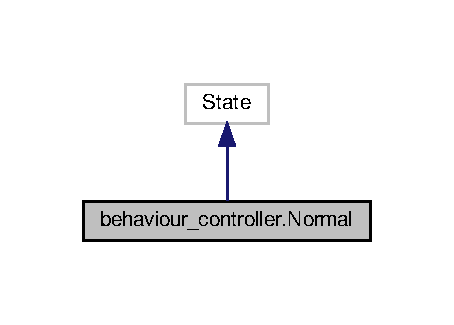
\includegraphics[width=218pt]{classbehaviour__controller_1_1Normal__inherit__graph}
\end{center}
\end{figure}


Collaboration diagram for behaviour\+\_\+controller.\+Normal\+:\nopagebreak
\begin{figure}[H]
\begin{center}
\leavevmode
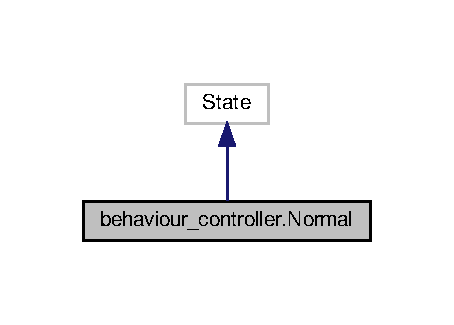
\includegraphics[width=218pt]{classbehaviour__controller_1_1Normal__coll__graph}
\end{center}
\end{figure}
\subsection*{Public Member Functions}
\begin{DoxyCompactItemize}
\item 
def \hyperlink{classbehaviour__controller_1_1Normal_a4ab0fac79d6253442382a49e4388daf5}{\+\_\+\+\_\+init\+\_\+\+\_\+} (self)
\begin{DoxyCompactList}\small\item\em method init \end{DoxyCompactList}\item 
def \hyperlink{classbehaviour__controller_1_1Normal_a92056bce8fb8c056227de8134c0b2360}{execute} (self, userdata)
\begin{DoxyCompactList}\small\item\em method execute \end{DoxyCompactList}\item 
def \hyperlink{classbehaviour__controller_1_1Normal_afc29036dc946ac6c711417da07ca8690}{get\+\_\+command} (self, command)
\begin{DoxyCompactList}\small\item\em method get\+\_\+command \end{DoxyCompactList}\end{DoxyCompactItemize}
\subsection*{Public Attributes}
\begin{DoxyCompactItemize}
\item 
\hyperlink{classbehaviour__controller_1_1Normal_a52be6081cfd23a5661fb4304774f1d17}{command\+\_\+received}
\begin{DoxyCompactList}\small\item\em check if a voice command is received \end{DoxyCompactList}\item 
\mbox{\Hypertarget{classbehaviour__controller_1_1Normal_ac9e8f54b79853ae9dcb0c5b4473aaab5}\label{classbehaviour__controller_1_1Normal_ac9e8f54b79853ae9dcb0c5b4473aaab5}} 
{\bfseries rate}
\end{DoxyCompactItemize}


\subsection{Detailed Description}
class state \hyperlink{classbehaviour__controller_1_1Normal}{Normal} 

normal behaviour of the pet 

\subsection{Constructor \& Destructor Documentation}
\mbox{\Hypertarget{classbehaviour__controller_1_1Normal_a4ab0fac79d6253442382a49e4388daf5}\label{classbehaviour__controller_1_1Normal_a4ab0fac79d6253442382a49e4388daf5}} 
\index{behaviour\+\_\+controller\+::\+Normal@{behaviour\+\_\+controller\+::\+Normal}!\+\_\+\+\_\+init\+\_\+\+\_\+@{\+\_\+\+\_\+init\+\_\+\+\_\+}}
\index{\+\_\+\+\_\+init\+\_\+\+\_\+@{\+\_\+\+\_\+init\+\_\+\+\_\+}!behaviour\+\_\+controller\+::\+Normal@{behaviour\+\_\+controller\+::\+Normal}}
\subsubsection{\texorpdfstring{\+\_\+\+\_\+init\+\_\+\+\_\+()}{\_\_init\_\_()}}
{\footnotesize\ttfamily def behaviour\+\_\+controller.\+Normal.\+\_\+\+\_\+init\+\_\+\+\_\+ (\begin{DoxyParamCaption}\item[{}]{self }\end{DoxyParamCaption})}



method init 

state initialization 

\subsection{Member Function Documentation}
\mbox{\Hypertarget{classbehaviour__controller_1_1Normal_a92056bce8fb8c056227de8134c0b2360}\label{classbehaviour__controller_1_1Normal_a92056bce8fb8c056227de8134c0b2360}} 
\index{behaviour\+\_\+controller\+::\+Normal@{behaviour\+\_\+controller\+::\+Normal}!execute@{execute}}
\index{execute@{execute}!behaviour\+\_\+controller\+::\+Normal@{behaviour\+\_\+controller\+::\+Normal}}
\subsubsection{\texorpdfstring{execute()}{execute()}}
{\footnotesize\ttfamily def behaviour\+\_\+controller.\+Normal.\+execute (\begin{DoxyParamCaption}\item[{}]{self,  }\item[{}]{userdata }\end{DoxyParamCaption})}



method execute 

state execution \mbox{\Hypertarget{classbehaviour__controller_1_1Normal_afc29036dc946ac6c711417da07ca8690}\label{classbehaviour__controller_1_1Normal_afc29036dc946ac6c711417da07ca8690}} 
\index{behaviour\+\_\+controller\+::\+Normal@{behaviour\+\_\+controller\+::\+Normal}!get\+\_\+command@{get\+\_\+command}}
\index{get\+\_\+command@{get\+\_\+command}!behaviour\+\_\+controller\+::\+Normal@{behaviour\+\_\+controller\+::\+Normal}}
\subsubsection{\texorpdfstring{get\+\_\+command()}{get\_command()}}
{\footnotesize\ttfamily def behaviour\+\_\+controller.\+Normal.\+get\+\_\+command (\begin{DoxyParamCaption}\item[{}]{self,  }\item[{}]{command }\end{DoxyParamCaption})}



method get\+\_\+command 

subscriber callback for voice command 

\subsection{Member Data Documentation}
\mbox{\Hypertarget{classbehaviour__controller_1_1Normal_a52be6081cfd23a5661fb4304774f1d17}\label{classbehaviour__controller_1_1Normal_a52be6081cfd23a5661fb4304774f1d17}} 
\index{behaviour\+\_\+controller\+::\+Normal@{behaviour\+\_\+controller\+::\+Normal}!command\+\_\+received@{command\+\_\+received}}
\index{command\+\_\+received@{command\+\_\+received}!behaviour\+\_\+controller\+::\+Normal@{behaviour\+\_\+controller\+::\+Normal}}
\subsubsection{\texorpdfstring{command\+\_\+received}{command\_received}}
{\footnotesize\ttfamily behaviour\+\_\+controller.\+Normal.\+command\+\_\+received}



check if a voice command is received 

go to sleep at random (1/300 chances per iteration -\/$>$ 100 iterations per second -\/$>$ 1/3 chance per second passed in \hyperlink{classbehaviour__controller_1_1Normal}{Normal} state) 

The documentation for this class was generated from the following file\+:\begin{DoxyCompactItemize}
\item 
behaviour\+\_\+controller.\+py\end{DoxyCompactItemize}

\hypertarget{classpet__map_1_1PetMap}{}\section{pet\+\_\+map.\+Pet\+Map Class Reference}
\label{classpet__map_1_1PetMap}\index{pet\+\_\+map.\+Pet\+Map@{pet\+\_\+map.\+Pet\+Map}}


class Map  


\subsection*{Public Member Functions}
\begin{DoxyCompactItemize}
\item 
def \hyperlink{classpet__map_1_1PetMap_a8235a0010f925e43233c2133291c5f62}{\+\_\+\+\_\+init\+\_\+\+\_\+} (self)
\begin{DoxyCompactList}\small\item\em The constructor. \end{DoxyCompactList}\item 
def \hyperlink{classpet__map_1_1PetMap_a98a355ec64fdefbf2ff773d7904995d1}{update\+Map} (self, x, y)
\begin{DoxyCompactList}\small\item\em method update\+Map \end{DoxyCompactList}\end{DoxyCompactItemize}
\subsection*{Public Attributes}
\begin{DoxyCompactItemize}
\item 
\mbox{\Hypertarget{classpet__map_1_1PetMap_ab383dd014e2cb6fc75d2f19187f9c4df}\label{classpet__map_1_1PetMap_ab383dd014e2cb6fc75d2f19187f9c4df}} 
{\bfseries dimX}
\item 
\mbox{\Hypertarget{classpet__map_1_1PetMap_a138655b51dc4292b6426228df9cb951b}\label{classpet__map_1_1PetMap_a138655b51dc4292b6426228df9cb951b}} 
{\bfseries dimY}
\item 
\mbox{\Hypertarget{classpet__map_1_1PetMap_a1f2cb698135b8ba1ab7fe412a7a49276}\label{classpet__map_1_1PetMap_a1f2cb698135b8ba1ab7fe412a7a49276}} 
{\bfseries homeX}
\item 
\mbox{\Hypertarget{classpet__map_1_1PetMap_a83c61ed1b1e7ec7ef258e745b3138a3f}\label{classpet__map_1_1PetMap_a83c61ed1b1e7ec7ef258e745b3138a3f}} 
{\bfseries homeY}
\item 
\mbox{\Hypertarget{classpet__map_1_1PetMap_a9034a42582a94ad1075c446b8172403a}\label{classpet__map_1_1PetMap_a9034a42582a94ad1075c446b8172403a}} 
{\bfseries actualX}
\item 
\mbox{\Hypertarget{classpet__map_1_1PetMap_a5f859151207f6bd78a8f269e522963f2}\label{classpet__map_1_1PetMap_a5f859151207f6bd78a8f269e522963f2}} 
{\bfseries actualY}
\end{DoxyCompactItemize}


\subsection{Detailed Description}
class Map 

Map structure definition and functions 

\subsection{Constructor \& Destructor Documentation}
\mbox{\Hypertarget{classpet__map_1_1PetMap_a8235a0010f925e43233c2133291c5f62}\label{classpet__map_1_1PetMap_a8235a0010f925e43233c2133291c5f62}} 
\index{pet\+\_\+map\+::\+Pet\+Map@{pet\+\_\+map\+::\+Pet\+Map}!\+\_\+\+\_\+init\+\_\+\+\_\+@{\+\_\+\+\_\+init\+\_\+\+\_\+}}
\index{\+\_\+\+\_\+init\+\_\+\+\_\+@{\+\_\+\+\_\+init\+\_\+\+\_\+}!pet\+\_\+map\+::\+Pet\+Map@{pet\+\_\+map\+::\+Pet\+Map}}
\subsubsection{\texorpdfstring{\+\_\+\+\_\+init\+\_\+\+\_\+()}{\_\_init\_\_()}}
{\footnotesize\ttfamily def pet\+\_\+map.\+Pet\+Map.\+\_\+\+\_\+init\+\_\+\+\_\+ (\begin{DoxyParamCaption}\item[{}]{self }\end{DoxyParamCaption})}



The constructor. 


\begin{DoxyParams}{Parameters}
{\em self} & The object pointer \\
\hline
\end{DoxyParams}


\subsection{Member Function Documentation}
\mbox{\Hypertarget{classpet__map_1_1PetMap_a98a355ec64fdefbf2ff773d7904995d1}\label{classpet__map_1_1PetMap_a98a355ec64fdefbf2ff773d7904995d1}} 
\index{pet\+\_\+map\+::\+Pet\+Map@{pet\+\_\+map\+::\+Pet\+Map}!update\+Map@{update\+Map}}
\index{update\+Map@{update\+Map}!pet\+\_\+map\+::\+Pet\+Map@{pet\+\_\+map\+::\+Pet\+Map}}
\subsubsection{\texorpdfstring{update\+Map()}{updateMap()}}
{\footnotesize\ttfamily def pet\+\_\+map.\+Pet\+Map.\+update\+Map (\begin{DoxyParamCaption}\item[{}]{self,  }\item[{}]{x,  }\item[{}]{y }\end{DoxyParamCaption})}



method update\+Map 


\begin{DoxyParams}{Parameters}
{\em x} & X position \\
\hline
{\em y} & Y position \\
\hline
\end{DoxyParams}


The documentation for this class was generated from the following file\+:\begin{DoxyCompactItemize}
\item 
pet\+\_\+map.\+py\end{DoxyCompactItemize}

\hypertarget{classbehaviour__controller_1_1Play}{}\section{behaviour\+\_\+controller.\+Play Class Reference}
\label{classbehaviour__controller_1_1Play}\index{behaviour\+\_\+controller.\+Play@{behaviour\+\_\+controller.\+Play}}


class state \hyperlink{classbehaviour__controller_1_1Play}{Play}  




Inheritance diagram for behaviour\+\_\+controller.\+Play\+:\nopagebreak
\begin{figure}[H]
\begin{center}
\leavevmode
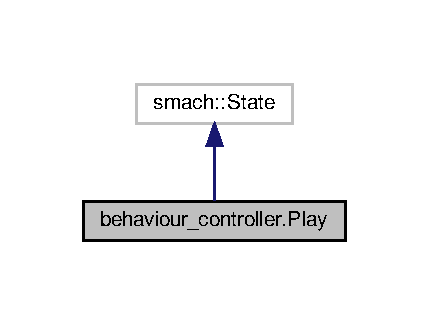
\includegraphics[width=206pt]{classbehaviour__controller_1_1Play__inherit__graph}
\end{center}
\end{figure}


Collaboration diagram for behaviour\+\_\+controller.\+Play\+:\nopagebreak
\begin{figure}[H]
\begin{center}
\leavevmode
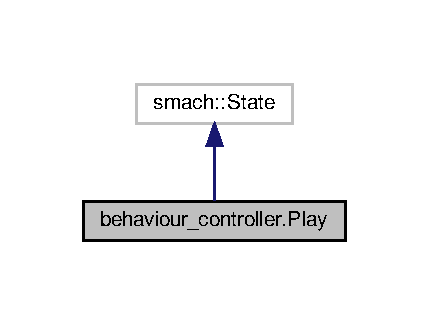
\includegraphics[width=206pt]{classbehaviour__controller_1_1Play__coll__graph}
\end{center}
\end{figure}
\subsection*{Public Member Functions}
\begin{DoxyCompactItemize}
\item 
def \hyperlink{classbehaviour__controller_1_1Play_a90fdc5f3993b7d5f4a65effec6a38965}{\+\_\+\+\_\+init\+\_\+\+\_\+} (self)
\begin{DoxyCompactList}\small\item\em method init \end{DoxyCompactList}\item 
def \hyperlink{classbehaviour__controller_1_1Play_af9a8184754ae235cf9a065392c0a8227}{execute} (self, userdata)
\begin{DoxyCompactList}\small\item\em method execute \end{DoxyCompactList}\item 
\mbox{\Hypertarget{classbehaviour__controller_1_1Play_a2f5b362cda5f127257507b259387d14c}\label{classbehaviour__controller_1_1Play_a2f5b362cda5f127257507b259387d14c}} 
def \hyperlink{classbehaviour__controller_1_1Play_a2f5b362cda5f127257507b259387d14c}{get\+\_\+position} (self, position)
\begin{DoxyCompactList}\small\item\em method get\+\_\+position subscriber callback, gets actual position of the robot \end{DoxyCompactList}\end{DoxyCompactItemize}
\subsection*{Public Attributes}
\begin{DoxyCompactItemize}
\item 
\mbox{\Hypertarget{classbehaviour__controller_1_1Play_af5b837d4d0897f22ab4c3c2d1c889539}\label{classbehaviour__controller_1_1Play_af5b837d4d0897f22ab4c3c2d1c889539}} 
{\bfseries position}
\item 
\mbox{\Hypertarget{classbehaviour__controller_1_1Play_aeefa0f6436617de2c6ffb6cfb18f329e}\label{classbehaviour__controller_1_1Play_aeefa0f6436617de2c6ffb6cfb18f329e}} 
{\bfseries rate}
\end{DoxyCompactItemize}


\subsection{Detailed Description}
class state \hyperlink{classbehaviour__controller_1_1Play}{Play} 

\hyperlink{classbehaviour__controller_1_1Play}{Play} behaviour of the pet 

\subsection{Constructor \& Destructor Documentation}
\mbox{\Hypertarget{classbehaviour__controller_1_1Play_a90fdc5f3993b7d5f4a65effec6a38965}\label{classbehaviour__controller_1_1Play_a90fdc5f3993b7d5f4a65effec6a38965}} 
\index{behaviour\+\_\+controller\+::\+Play@{behaviour\+\_\+controller\+::\+Play}!\+\_\+\+\_\+init\+\_\+\+\_\+@{\+\_\+\+\_\+init\+\_\+\+\_\+}}
\index{\+\_\+\+\_\+init\+\_\+\+\_\+@{\+\_\+\+\_\+init\+\_\+\+\_\+}!behaviour\+\_\+controller\+::\+Play@{behaviour\+\_\+controller\+::\+Play}}
\subsubsection{\texorpdfstring{\+\_\+\+\_\+init\+\_\+\+\_\+()}{\_\_init\_\_()}}
{\footnotesize\ttfamily def behaviour\+\_\+controller.\+Play.\+\_\+\+\_\+init\+\_\+\+\_\+ (\begin{DoxyParamCaption}\item[{}]{self }\end{DoxyParamCaption})}



method init 

state initialization 

\subsection{Member Function Documentation}
\mbox{\Hypertarget{classbehaviour__controller_1_1Play_af9a8184754ae235cf9a065392c0a8227}\label{classbehaviour__controller_1_1Play_af9a8184754ae235cf9a065392c0a8227}} 
\index{behaviour\+\_\+controller\+::\+Play@{behaviour\+\_\+controller\+::\+Play}!execute@{execute}}
\index{execute@{execute}!behaviour\+\_\+controller\+::\+Play@{behaviour\+\_\+controller\+::\+Play}}
\subsubsection{\texorpdfstring{execute()}{execute()}}
{\footnotesize\ttfamily def behaviour\+\_\+controller.\+Play.\+execute (\begin{DoxyParamCaption}\item[{}]{self,  }\item[{}]{userdata }\end{DoxyParamCaption})}



method execute 

state execution 

The documentation for this class was generated from the following file\+:\begin{DoxyCompactItemize}
\item 
behaviour\+\_\+controller.\+py\end{DoxyCompactItemize}

\hypertarget{classbehaviour__controller_1_1Sleep}{}\section{behaviour\+\_\+controller.\+Sleep Class Reference}
\label{classbehaviour__controller_1_1Sleep}\index{behaviour\+\_\+controller.\+Sleep@{behaviour\+\_\+controller.\+Sleep}}


class state \hyperlink{classbehaviour__controller_1_1Sleep}{Sleep}  




Inheritance diagram for behaviour\+\_\+controller.\+Sleep\+:\nopagebreak
\begin{figure}[H]
\begin{center}
\leavevmode
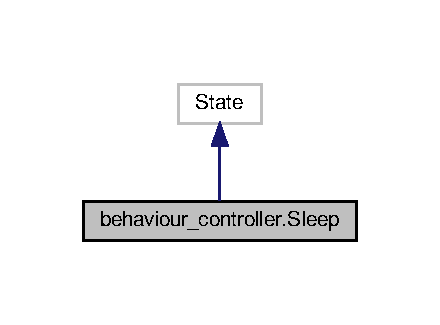
\includegraphics[width=211pt]{classbehaviour__controller_1_1Sleep__inherit__graph}
\end{center}
\end{figure}


Collaboration diagram for behaviour\+\_\+controller.\+Sleep\+:\nopagebreak
\begin{figure}[H]
\begin{center}
\leavevmode
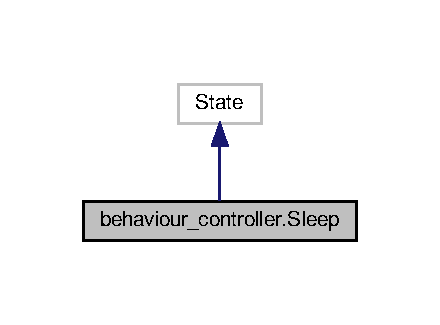
\includegraphics[width=211pt]{classbehaviour__controller_1_1Sleep__coll__graph}
\end{center}
\end{figure}
\subsection*{Public Member Functions}
\begin{DoxyCompactItemize}
\item 
def \hyperlink{classbehaviour__controller_1_1Sleep_afb1c72731d2499a8930ee354f37ca7ad}{\+\_\+\+\_\+init\+\_\+\+\_\+} (self)
\begin{DoxyCompactList}\small\item\em method init \end{DoxyCompactList}\item 
def \hyperlink{classbehaviour__controller_1_1Sleep_ae087af71e4af7b6a0967ddcaeecfe346}{execute} (self, userdata)
\begin{DoxyCompactList}\small\item\em method execute \end{DoxyCompactList}\item 
def \hyperlink{classbehaviour__controller_1_1Sleep_aebc97332fedcc5dc6f72c799d002088f}{get\+\_\+position} (self, \hyperlink{classbehaviour__controller_1_1Sleep_afef48330ea2405eb8cbe75e642e7dd59}{position})
\begin{DoxyCompactList}\small\item\em method get\+\_\+position \end{DoxyCompactList}\end{DoxyCompactItemize}
\subsection*{Public Attributes}
\begin{DoxyCompactItemize}
\item 
\mbox{\Hypertarget{classbehaviour__controller_1_1Sleep_afef48330ea2405eb8cbe75e642e7dd59}\label{classbehaviour__controller_1_1Sleep_afef48330ea2405eb8cbe75e642e7dd59}} 
\hyperlink{classbehaviour__controller_1_1Sleep_afef48330ea2405eb8cbe75e642e7dd59}{position}
\begin{DoxyCompactList}\small\item\em get the timescale parameter to adjust simulation speed \end{DoxyCompactList}\item 
\mbox{\Hypertarget{classbehaviour__controller_1_1Sleep_a33c3cb4863818478656fa80ea10a7318}\label{classbehaviour__controller_1_1Sleep_a33c3cb4863818478656fa80ea10a7318}} 
{\bfseries rate}
\end{DoxyCompactItemize}


\subsection{Detailed Description}
class state \hyperlink{classbehaviour__controller_1_1Sleep}{Sleep} 

\hyperlink{classbehaviour__controller_1_1Sleep}{Sleep} behaviour of the pet 

\subsection{Constructor \& Destructor Documentation}
\mbox{\Hypertarget{classbehaviour__controller_1_1Sleep_afb1c72731d2499a8930ee354f37ca7ad}\label{classbehaviour__controller_1_1Sleep_afb1c72731d2499a8930ee354f37ca7ad}} 
\index{behaviour\+\_\+controller\+::\+Sleep@{behaviour\+\_\+controller\+::\+Sleep}!\+\_\+\+\_\+init\+\_\+\+\_\+@{\+\_\+\+\_\+init\+\_\+\+\_\+}}
\index{\+\_\+\+\_\+init\+\_\+\+\_\+@{\+\_\+\+\_\+init\+\_\+\+\_\+}!behaviour\+\_\+controller\+::\+Sleep@{behaviour\+\_\+controller\+::\+Sleep}}
\subsubsection{\texorpdfstring{\+\_\+\+\_\+init\+\_\+\+\_\+()}{\_\_init\_\_()}}
{\footnotesize\ttfamily def behaviour\+\_\+controller.\+Sleep.\+\_\+\+\_\+init\+\_\+\+\_\+ (\begin{DoxyParamCaption}\item[{}]{self }\end{DoxyParamCaption})}



method init 

state initialization 

\subsection{Member Function Documentation}
\mbox{\Hypertarget{classbehaviour__controller_1_1Sleep_ae087af71e4af7b6a0967ddcaeecfe346}\label{classbehaviour__controller_1_1Sleep_ae087af71e4af7b6a0967ddcaeecfe346}} 
\index{behaviour\+\_\+controller\+::\+Sleep@{behaviour\+\_\+controller\+::\+Sleep}!execute@{execute}}
\index{execute@{execute}!behaviour\+\_\+controller\+::\+Sleep@{behaviour\+\_\+controller\+::\+Sleep}}
\subsubsection{\texorpdfstring{execute()}{execute()}}
{\footnotesize\ttfamily def behaviour\+\_\+controller.\+Sleep.\+execute (\begin{DoxyParamCaption}\item[{}]{self,  }\item[{}]{userdata }\end{DoxyParamCaption})}



method execute 

state execution \mbox{\Hypertarget{classbehaviour__controller_1_1Sleep_aebc97332fedcc5dc6f72c799d002088f}\label{classbehaviour__controller_1_1Sleep_aebc97332fedcc5dc6f72c799d002088f}} 
\index{behaviour\+\_\+controller\+::\+Sleep@{behaviour\+\_\+controller\+::\+Sleep}!get\+\_\+position@{get\+\_\+position}}
\index{get\+\_\+position@{get\+\_\+position}!behaviour\+\_\+controller\+::\+Sleep@{behaviour\+\_\+controller\+::\+Sleep}}
\subsubsection{\texorpdfstring{get\+\_\+position()}{get\_position()}}
{\footnotesize\ttfamily def behaviour\+\_\+controller.\+Sleep.\+get\+\_\+position (\begin{DoxyParamCaption}\item[{}]{self,  }\item[{}]{position }\end{DoxyParamCaption})}



method get\+\_\+position 

subscriber callback, gets actual position of the robot 

The documentation for this class was generated from the following file\+:\begin{DoxyCompactItemize}
\item 
behaviour\+\_\+controller.\+py\end{DoxyCompactItemize}

%--- End generated contents ---

% Index
\backmatter
\newpage
\phantomsection
\clearemptydoublepage
\addcontentsline{toc}{chapter}{Index}
\printindex

\end{document}
